\documentclass[preprint,10pt,a4paper]{elsarticle}

%------------------------------------------------------------------------------
%	REQUIRED PACKAGES AND  CONFIGURATIONS
%------------------------------------------------------------------------------
% PACKAGES FOR TITLES
\usepackage{titlesec}
\usepackage[dvipsnames]{xcolor}
\newcommand{\tommi}[1]{\textcolor{blue}{#1}}
\newcommand{\elisa}[1]{\textcolor{red}{#1}}
\newcommand{\gas}[1]{\textcolor{green}{#1}}


% PACKAGES FOR LANGUAGE AND FONT
\usepackage[utf8]{inputenc}
\usepackage[english]{babel}
\usepackage[T1]{fontenc} % Font encoding
\usepackage{verbatim}
\usepackage{dutchcal}
% PACKAGES FOR IMAGES
\usepackage{graphicx}
\usepackage{adjustbox}
\graphicspath{{Images/}} % Path for images' folder
\usepackage{eso-pic} % For the background picture on the title page
\usepackage{subfig} % Numbered and caption subfigures using \subfloat
\usepackage{caption} % Coloured captions
\usepackage{transparent}

\usepackage{booktabs}

% STANDARD MATH PACKAGES
\usepackage{amsmath}
\usepackage{amsthm}
\usepackage{bm}
\usepackage[overload]{empheq}  % For braced-style systems of equations

% PACKAGES FOR TABLES
\usepackage{tabularx}
\usepackage{longtable} % tables that can span several pages
\usepackage{colortbl}

% PACKAGES FOR ALGORITHMS (PSEUDO-CODE)
%\usepackage[noend]{algpseudocode}
%\usepackage{algorithm}

%\newcommand{\pushcode}[1][1]{\hskip\dimexpr#1\algorithmicindent\relax}
\usepackage{algorithm2e}

% permette di scrivere "text" 
\usepackage[autostyle]{csquotes}
\MakeOuterQuote{"}

%MATH
\usepackage{amssymb}
\usepackage{amsmath}

% PACKAGES FOR REFERENCES & BIBLIOGRAPHY
\usepackage[colorlinks=true,linkcolor=black,anchorcolor=black,citecolor=black,filecolor=black,menucolor=black,runcolor=black,urlcolor=black]{hyperref} % Adds clickable links at references
\usepackage{cleveref}
%\usepackage[square, numbers, sort&compress]{natbib} % Square brackets, citing references with numbers, citations sorted by appearance in the text and compressed
\bibliographystyle{plain} % You may use a different style adapted to your field

\usepackage{tabularx}

% PACKAGES FOR THE APPENDIX
\usepackage{appendix}

% PACKAGES FOR ITEMIZE & ENUMERATES 
\usepackage{enumitem}

\usepackage{smartdiagram}

% OTHER PACKAGES
\usepackage{amsthm,thmtools,xcolor} % Coloured "Theorem"
\usepackage{comment} % Comment part of code
\usepackage{fancyhdr} % Fancy headers and footers
\usepackage{lipsum} % Insert dummy text
\usepackage{tcolorbox} % Create coloured boxes (e.g. the one for the key-words)
\usepackage{xcolor}
\usepackage{stfloats} % Correct position of the tables
\usepackage{tikz}
\usepackage{pgfplots}

\usepgfplotslibrary{external}
\pgfplotsset{compat=1.14}

\newcommand{\approach}{ALIF\xspace}

%\title{Tune anomaly detection towards the target: Active Isolation Forest with leaf fixers}
\title{Active Learning-based Isolation Forest (\approach): Enhancing Anomaly Detection in Decision Support Systems}


    
\author[inst1]{Elisa Marcelli}       
\author[inst1]{Tommaso Barbariol}
\address[inst1]{Department of Information Engineering, University of Padova, Via Giovanni Gradenigo 6, Padova, 35131, PD, Italy}
%\affiliation[inst1]{organization={Department of Information Engineering, University of Padova},%Department and Organization
  %          addressline={Via Giovanni Gradenigo 6}, 
    %        city={Padova},
      %      postcode={35131}, 
      %      state={PD},
        %    country={Italy}}

\author[inst1,inst2]{Gian Antonio Susto}

%\affiliation[inst2]{organization={Human Inspired Technology Research Centre, University of Padova},%Department and Organization
  %          addressline={Via Luigi Luzzatti 4}, 
    %        city={Padova},
      %      postcode={35121}, 
        %    state={PD},
          %  country={Italy}}
 \address[inst2]{Human Inspired Technology Research Centre, University of Padova, Via Luigi Luzzatti, Padova, 35121, PD, Italy}        
\journal{Information Sciences}
\begin{document}

\begin{abstract} % of up to 200 words -> 200
The detection of anomalous behaviours is an emerging need in many applications, particularly in contexts where security and reliability are critical aspects. While the definition of anomaly strictly depends on the domain framework, it is often impractical or too time consuming to obtain a fully labelled dataset. The use of unsupervised models to overcome the lack of labels often fails to catch domain specific anomalies as they rely on general definitions of outlier. This paper suggests a new active learning based approach, \approach, to solve this problem by reducing the number of required labels and tuning the detector towards the definition of anomaly provided by the user.
%through the given labels. %\gas{Forse dovremmo menzionare anche la crescente disponibilità di approcci unsupervised nei sistemi di supporto alle decisioni, che delinea un nuovo scenario, poco esplorato in letteratura, di aver a disposizione - dopo la creazione di un sistema di AD - feedback da parte dell'utente, in maniera semplice/'non costosa'.} 
%\tommi{PROPOSTA: The proposed model exploits the feedback the user of a Decision Support System (DSS) provides during its operation. Indeed \approach is able to enhance the capabilities of DSS that usually rely on unsupervised models and are not able to continuously update their models.}
%\elisa{Due to the lack of available labels as well as to the often excessive cost needed to get them, anomaly detection has strongly adopted unsupervised approaches. In a Decision Support System, a user constantly interacts with the system, making the final decisions and providing feedback. In this case, \approach proposes a novel inexpensive way to modify the model based on the user's feedback.}
The proposed approach is particularly appealing in the presence of a Decision Support System (DSS), a case that is increasingly popular in real-world scenarios. While it is common that DSS embedded with anomaly detection capabilities rely on unsupervised models, they don't have a way to improve their performance: \approach is able to enhance the capabilities of DSS by exploiting the user feedback during common operations. %More in general, 
\approach is a lightweight modification of the popular Isolation Forest that proved superior performances %in terms of average precision score 
with respect to other state-of-art algorithms in a multitude of real anomaly detection datasets. 

% we propose ALIF by interacting with the user through the DSS is able to collect useful informations to update the model

\end{abstract}

\begin{keyword}
Active Learning \sep Anomaly Detection \sep Decision Support System \sep Industry 4.0 \sep Isolation Forest \sep Machine Learning \sep Weakly Supervised Learning
\end{keyword}
\maketitle

%\tommi{Bisogna che facciamo una scaletta di tutto il paper:}
%\begin{itemize}
 %   \item il machine learning è utile in vari contesti come quello industriale
 %   \item l'anomaly detection è un task molto importante
  %  \item le anomalie sono domain-specific
   % \item allora sarebbe bello avere tutti i dati ettichettati
%    \item è troppo costoso, nella pratica si fa tutto non supervisionato
 %   \item sarebbe bello però avere delle informazioni in modo da guidare il detector verso le anomalie domain specific
  %  \item l'active learning viene in nostro aiuto
   % \item esprimiamo la nostra idea
    %\item struttura del paper
%\end{itemize}

%\begin{itemize}
%\item anomaly detection
%\item isolation forest
%\item active learning
%\end{itemize}

%\begin{itemize}
%\item nostra query strategy
%\item nostra fixing strategy
%\end{itemize}

%%%%%%%%%%%%%%%%%%%%%%%%%%%%%%%%%%%%%%%%%%%%%%%%%%
\section{Introduction}
\label{main:sec:introduction}
%%%%%%%%%%%%%%%%%%%%%%%%%%%%%%%%%%%%%%%%%%%%%%%%%%

\glsresetall

% \ljh{Just a draft. need polishing and proofreading}
A \gls{np}~\citep{garnelo2018conditional,garnelo2018neural} meta-learns a stochastic process describing the relationship between inputs and outputs in a given data stream, where each task in the data stream consists of a meta-training set of input-output pairs and also a meta-validation set. The \gls{np} then defines an implicit stochastic process whose functional form is determined by a neural network taking the meta-training set as an input, and the parameters of the neural network are optimized to maximize the predictive likelihood for the meta-validation set. This approach is philosophically different from the traditional learning pipeline where one would first elicit a stochastic process from the known class of models (e.g., \glspl{gp}) and hope that it describes the data well. An ideal \gls{np} would assume minimal inductive biases and learn as much as possible from the data. In this regard, \glspl{np} can be framed as a ``data-driven'' way of choosing proper stochastic processes.

 An important design choice for a \gls{np} model is how to capture the uncertainty in the random functions drawn from stochastic processes. When mapping the meta-training set into a function, one might employ a deterministic mapping as in \citet{garnelo2018conditional}. However, it is more natural to assume that there may be multiple plausible functions that might have generated the given data, and thus encode the functional (epistemic) uncertainty as a part of the \gls{np} model. \citet{garnelo2018neural} later proposed to map the meta-training set into a fixed dimensional \emph{global latent variable} with a Gaussian posterior approximation. While this improves upon the vanilla model without such a latent variable~\citep{le2018empirical}, expressing the functional uncertainty only through the Gaussian approximated latent variable has been reported to be a bottleneck~\citep{louizos2019functional}. To this end, \citet{lee2020bootstrapping} and \citet{lee2022neural} propose to apply bootstrap to the meta-training set to use the uncertainty arising from the population distribution as a source for the functional uncertainty.

In this paper, we take a rather different approach to define the functional uncertainty for \glspl{np}. Specifically, we utilize the martingale posterior distribution~\citep{fong2021martingale}, a recently developed alternative to conventional Bayesian inference. In the martingale posterior, instead of eliciting a likelihood-prior pair and inferring the Bayesian posterior, we elicit a joint predictive distribution on future data given observed data. Under suitable conditions on such a predictive distribution, it can be shown that the uncertainty due to the generated future data indeed corresponds to the uncertainty of the Bayesian posterior. Following this, we endow a \gls{np} with a joint predictive distribution defined through neural networks and derive the functional uncertainty as the uncertainty arising when mapping the randomly generated future data to the functions. Compared to the previous approaches of either explicitly positing a finite-dimensional variable encoding the functional uncertainty or deriving it from a population distribution, our method makes minimal assumptions about the predictive distribution and gives more freedom to the model to choose the proper form of uncertainty solely from the data. Due to the theory of martingale posteriors, our model guarantees the existence of the martingale posterior corresponding to the valid Bayesian posterior of an implicitly defined parameter. 
% \ed{Does the following make sense: }
Furthermore, working in the space of future observations allows us to incorporate the latent functional uncertainty path with deterministic path in a more natural manner.
% \ljh{It would be good to have more concrete motivation to prefer the martingale posteriors over conventional Bayesian inference; what would be an advantage of doing that, aside from the fact that we don't need to choose likelihood and prior?} \ed{I'll have a think about this, and will also do some proofreading. Because of the time difference and my job hours, timing might be a bit tricky tomorrow. When would be the best time for me to proofread?}

We name our extension of \glspl{np} with the joint predictive generative models as the \gls{mpnp}. Throughout the paper, we propose an efficient neural network architecture for the generative model that is easy to implement, flexible, and yet guarantees the existence of the martingale posterior. We also propose a training scheme to stably learn the parameters of \glspl{mpnp}. Using various synthetic and real-world regression tasks, we demonstrate that \gls{mpnp} significantly outperforms the previous \gls{np} variants in terms of predictive performance.





% \gls{npf}~\citep{garnelo2018conditional, garnelo2018neural} is a class of parametric models which defines stochastic processes over given data using neural networks.
% Unlike classical stochastic processes (e.g. \glspl{gp}), \gls{npf} learns to fit a proper stochastic processes from data under meta-learning framework.
% The deterministic version of \gls{npf}, \glspl{cnp}~\citep{garnelo2018conditional} deterministically map each dataset to a certain stochastic process which does not consider functional uncertainty.
% In order to compensate for this problem, \glspl{np}~\citep{garnelo2018neural} introduce a global latent variable which captures functional uncertainty.
% \citet{le2018empirical} empirically shows that considering functional uncertainty in \glspl{np} improves the diversity in function realizations and the predictive performance for data.

% Although \glspl{np} tries to capture functional uncertainty, there is some limitations for \glspl{np} to well capture uncertainty with a Gaussian latent variable.
% To overcome this problem, there are some prior works which applying advanced functional uncertainty modeling strategies~\citep{lee2020bootstrapping}\citep{lee2022neural} instead of a global latent variable.
% \gls{bnp}~\citep{lee2020bootstrapping} employs the residual bootstrapping strategy to make more robust uncertainty estimation even for the data-model mismatch situation. 
% However, \gls{bnp} requires a high computational cost compared to \gls{np} due to it's residual bootstrapping strategy.
% \gls{neubnp}~\citep{lee2022neural} employs the recent computationally efficient bootstrapping of the neural network called Neural Bootstrapper~\citep{shin2021neural}.
% However, \gls{neubnp} multiplies Dirichlet distributed random bootstrap weights to features of context dataset which disturbs model to well recovers the given dataset.

% This paper presents a novel extension of \gls{npf} which introduces functional uncertainty by changing posterior uncertainty on function parameters as predictive uncertainty on the unseen data conditional on the observed data...

\section{Related Works} \label{rel_works}

Offline RL (\cite{DBLP:journals/corr/abs-2005-01643, DBLP:journals/corr/abs-2402-13777}) enables an agent to learn control policies from datasets of environment transitions pre-collected by a behavior policy $\mu$, i.e., $\mathcal{D}_\mu = \{[(s_t^i, a_t^i, r_t^i)_{t=1}^T]_{i=1}^N\}$, circumventing the need for potentially expensive or unsafe online interactions. Model-free offline RL methods directly learn value/policy functions from \(\mathcal{D}_\mu\) but restrict the policy to remain close to \(\mu\) or to behave within the support of \(\mathcal{D}_\mu\). Offline Model-based RL (MBRL) methods, on the other hand, explicitly learn world models $\mathcal{M}_\theta$ from $\mathcal{D}_\mu$ (through supervised learning) and adopt $\mathcal{M}_\theta$ as a surrogate simulator, enabling the learned policy to possibly generalize to states beyond $\mathcal{D}_\mu$. Specifically, both planning methods (\cite{DBLP:conf/iclr/ArgensonD21, DBLP:conf/ijcai/ZhanZX22, DBLP:journals/ral/DiehlSKHB23}), such as MPC (\cite{garcia1989model}), and RL methods (\cite{DBLP:conf/nips/YuTYEZLFM20, DBLP:conf/nips/KidambiRNJ20, DBLP:conf/iclr/LuBPOR22, DBLP:conf/nips/YuKRRLF21, DBLP:conf/nips/GuoSG22}) can be applied on top of the learned $\mathcal{M}_\theta$. However, since $\mathcal{D}_\mu$ may not span the entire state-action space, $\mathcal{M}_\theta$ is unlikely to be globally accurate. Learning/Planning without any safeguards against such model inaccuracy can yield poor results. In this case, the authors of (\cite{DBLP:conf/nips/YuTYEZLFM20, DBLP:conf/nips/KidambiRNJ20, DBLP:conf/iclr/LuBPOR22}) propose learning an ensemble of world models, using ensemble-based uncertainty estimations to construct a pessimistic MDP (P-MDP), and learning a near-optimal policy atop it. Ideally, for any policy, the performance in the real environment is lower-bounded by the performance in the corresponding P-MDP (with high probability), thus avoiding being overly optimistic about an inaccurate model. For practical implementation of the P-MDP, \cite{DBLP:conf/iclr/LuBPOR22} conduct a thorough empirical study to compare a series of heuristics. However, none of these offline MBRL methods have modeled the problem as a BAMDP, even though Bayesian RL/planning provides a principled framework for handling model uncertainty. Additionally, with the learned model \(\mathcal{M}_\theta\), deep and broad search in the policy learning process is possible, but the offline RL methods introduced above have not attempted such search-based policy improvement.

Monte-Carlo Tree Search (MCTS, \cite{browne2012survey}) has been successfully integrated with RL, as exemplified by AlphaZero (\cite{DBLP:journals/corr/abs-1712-01815}) and MuZero (\cite{DBLP:journals/nature/SchrittwieserAH20}). These methods have achieved superhuman performance in domains requiring highly precise and sophisticated decision-making processes. 
AlphaZero relies on given world models, whereas MuZero learns the world model and policy simultaneously by interacting with the environment. Although there have been various extensions of MuZero (\cite{DBLP:conf/icml/HubertSABSS21, DBLP:conf/nips/SchrittwieserHM21, DBLP:conf/nips/YeLKAG21, DBLP:conf/iclr/DanihelkaGSS22, DBLP:conf/iclr/AntonoglouSOHS22, oren2022mcts, DBLP:journals/corr/abs-2305-17327, zhao2024a}), most algorithms are designed for online MBRL. According to \cite{DBLP:conf/nips/NiuPYLZRHLL23}, the applications of MuZero in offline learning, especially for continuous control in highly stochastic environments, which is our focus, still require significant improvement. Although search-based, MuZero learns a dynamics model and a reward model in a latent state space rather than the real state space, does not apply uncertainty estimation of the learned models as in usual offline MBRL methods, and does not adopt the Bayesian RL framework, making it fundamentally different from our algorithm design.

As mentioned in Section \ref{back}, Bayes-optimal planning is typically intractable. Approximate methods, such as (\cite{DBLP:conf/uai/AsmuthLLNW09, DBLP:conf/uai/SorgSL10, DBLP:conf/pkdd/CastroP10, asmuth2011approaching, DBLP:conf/icml/WangWHL12, DBLP:conf/adprl/FonteneauBM13, DBLP:journals/jair/GuezSD13, DBLP:journals/iet-cps/SladeSK20}) have been developed. As a representative work, BAMCP (\cite{DBLP:journals/jair/GuezSD13}) adopts MCTS for Bayes Adaptive planning and is shown to converge in probability to a near Bayes-optimal policy at the root node of the search tree. However, all these methods cannot be directly applied to large-scale MDPs with continuous state and action spaces. \cite{DBLP:conf/nips/GuezHSD14} and \cite{DBLP:journals/corr/abs-2010-15948} attempt to extend the use of BAMCP to scenarios with continuous states and actions using value/policy function approximations, but they replace MCTS with simple Monte Carlo rollouts (\cite{DBLP:journals/heuristics/BertsekasC99}) and do not utilize UCT (\cite{DBLP:conf/ecml/KocsisS06}). Tree search makes branches at each node in the tree, providing a more thorough look-ahead search than simple rollouts, and UCT, as an efficient exploration algorithm, is the basis for the convergence guarantee of BAMCP. Moreover, these planning algorithms are not designed for offline MBRL. How to incorporate search-based planning in the policy improvement stage of RL and how to handle the uncertainty of the learned world model require further exploration, which are shown in the following section.

\section{Proposed model: \approach}
\label{pm}
In this paper we present an adaptive anomaly detection model for fixing leaf depths according to labels received from domain experts.
The core idea of the proposed approach is presented in Algorithm \ref{alg_albif} and relies on developing an Isolation Forest based model in which the detector has the possibility to query domain experts for labels. In this iterative environment, once the Isolation Forest is fully grown, the algorithm can choose the points to be labeled and, based on the novel information achieved, its core structure is modified, in order to obtain a strong increase in the performance, with the use of only a limited number of labeled points. For every iteration, such modification only takes place in the external node containing the queried point, maintaining the main structure of the Isolation Forest untouched. In this way, the main goal is, given the novel information, to update the Isolation Forest structure, readjusting it based on the labeled points.  

%% ALGORITHM STYLE -- Released 8 April 1996
%    for LaTeX-2e
% Copyright -- 1994 Peter Williams
% E-mail Peter.Williams@dsto.defence.gov.au
\NeedsTeXFormat{LaTeX2e}
\ProvidesPackage{algorithm}
\typeout{Document Style `algorithm' - floating environment}

\RequirePackage{float}
\RequirePackage{ifthen}
\newcommand{\ALG@within}{nothing}
\newboolean{ALG@within}
\setboolean{ALG@within}{false}
\newcommand{\ALG@floatstyle}{ruled}
\newcommand{\ALG@name}{Algorithm}
\newcommand{\listalgorithmname}{List of \ALG@name s}

% Declare Options
% first appearance
\DeclareOption{plain}{
  \renewcommand{\ALG@floatstyle}{plain}
}
\DeclareOption{ruled}{
  \renewcommand{\ALG@floatstyle}{ruled}
}
\DeclareOption{boxed}{
  \renewcommand{\ALG@floatstyle}{boxed}
}
% then numbering convention
\DeclareOption{part}{
  \renewcommand{\ALG@within}{part}
  \setboolean{ALG@within}{true}
}
\DeclareOption{chapter}{
  \renewcommand{\ALG@within}{chapter}
  \setboolean{ALG@within}{true}
}
\DeclareOption{section}{
  \renewcommand{\ALG@within}{section}
  \setboolean{ALG@within}{true}
}
\DeclareOption{subsection}{
  \renewcommand{\ALG@within}{subsection}
  \setboolean{ALG@within}{true}
}
\DeclareOption{subsubsection}{
  \renewcommand{\ALG@within}{subsubsection}
  \setboolean{ALG@within}{true}
}
\DeclareOption{nothing}{
  \renewcommand{\ALG@within}{nothing}
  \setboolean{ALG@within}{true}
}
\DeclareOption*{\edef\ALG@name{\CurrentOption}}

% ALGORITHM
%
\ProcessOptions
\floatstyle{\ALG@floatstyle}
\ifthenelse{\boolean{ALG@within}}{
  \ifthenelse{\equal{\ALG@within}{part}}
     {\newfloat{algorithm}{htbp}{loa}[part]}{}
  \ifthenelse{\equal{\ALG@within}{chapter}}
     {\newfloat{algorithm}{htbp}{loa}[chapter]}{}
  \ifthenelse{\equal{\ALG@within}{section}}
     {\newfloat{algorithm}{htbp}{loa}[section]}{}
  \ifthenelse{\equal{\ALG@within}{subsection}}
     {\newfloat{algorithm}{htbp}{loa}[subsection]}{}
  \ifthenelse{\equal{\ALG@within}{subsubsection}}
     {\newfloat{algorithm}{htbp}{loa}[subsubsection]}{}
  \ifthenelse{\equal{\ALG@within}{nothing}}
     {\newfloat{algorithm}{htbp}{loa}}{}
}{
  \newfloat{algorithm}{htbp}{loa}
}
\floatname{algorithm}{\ALG@name}

%\newcommand{\listofalgorithms}{\listof{algorithm}{\listalgorithmname}}



\begin{algorithm}
\caption{\textit{\approach$((x^{\mathcal{s}},y^{\mathcal{s}}), X^{\mathcal{u}}, F)$}}\label{alg_albif}
\KwData{labeled point $(x^{\mathcal{s}},y^{\mathcal{s}})$, unlabeled dataset $X^{\mathcal{u}}$, forest $F$}
\KwResult{updated forest $F$, query point $x^{\mathcal{s}}$} 
 $F \gets$ \textit{LeafDepthUpdate}$((x^{\mathcal{s}},y^{\mathcal{s}})$, $F)$\;
     $H \gets$ \textit{GetDepthMatrix}$(X^{\mathcal{u}}$, $F)$\;
    $x^{\mathcal{s}} \gets$ \textit{GetQuery}$(H)$

\end{algorithm}

\begin{algorithm}
\caption{\textit{LeafDepthUpdate$((x^{\mathcal{s}},y^{\mathcal{s}})$, $F)$}}\label{alg_leafDepth}
\KwData{labeled point $(x^{\mathcal{s}},y^{\mathcal{s}})$, unlabeled dataset $X^{\mathcal{u}}$, forest $F$}
\KwResult{updated leaf $L$} 
\For{$T_t$ \text{in} $F$}{
        $L \gets \lambda_{T_t}(x^{\mathcal{s}})$ \;
        \If{$y_{\mathcal{s}}==$ \text{anomaly}}{$L_\mathcal{o} \gets L_\mathcal{o} + 1$ \;}
        \Else{$L_\mathcal{i} \gets L_\mathcal{i} + 1$ \;}
        $L_\mathcal{h} \gets  h^\mathcal{s}(k(L))$
}
\end{algorithm}


\begin{algorithm}
\caption{\textit{GetDepthMatrix$(X^{\mathcal{u}}, F)$}}\label{alg_DepthMatrix}
\KwData{unlabeled dataset $X^{\mathcal{u}}$, forest $F$}
\KwResult{updated leaf $L$} 
\For{$T_t$ \text{in} $F$}{
    \For{$x^{\mathcal{u}}_j$ \text{in} $X^{\mathcal{u}}$}{
            $L \gets \lambda_{T_t}(x^{\mathcal{u}}_j)$ \;
            $H_{jt} \gets  h^\mathcal{s}(k(L))$
    }
}
\end{algorithm}


Specifically, the proposed approach may be outlined as follows. Let $X=\{x^1,\dots, x^n\}$ be a generic training dataset, where $x^i \in \mathbb{R}^m$, $i=1,\dots,n$. First, the Isolation Forest algorithm is trained, leading to a forest $F=\{T_t\}_{t=1}^{n_T}$ of fixed number $n_T$ of fully grown iTrees. By construction, $T=\{L_l\}_{l=1}^{n_L}$ namely each tree $T$ is characterized by a variable number of leaves $L$. We use the following form to describe each leaf $L$:
$L=(L_\mathcal{p}, L_H, L_\mathcal{i}, L_\mathcal{o})$
where 
\begin{itemize}
    \item $L_\mathcal{p}$ defines the partition of $X$ made by $L$, describing where a leaf is located with respect to the input space;
    \item $L_\mathcal{h}$ is the depth of $L$;
    \item $L_\mathcal{i}$ refers to the number of normal points in $L$;
    \item $L_\mathcal{o}$ specifies the amount of anomalies contained in $L$.
\end{itemize}
As a direct consequence, initially each data $x \in X$ is assigned with the corresponding average path length $E(h^\mathcal{u}(x))$ and anomaly score $a_\psi(x)$ as computed by the Isolation Forest. 
%aggiungere qui la quaterna? o più sotto?

From this step, the proposed iterative active learning approach can start. At each iteration, a point $x^{\mathcal{s}}$ is selected and the corresponding true label $y_{\mathcal{s}}$ is requested. Accordingly, each iTree $T$ is investigated, determining the leaf where the queried point lies, and modified as a result. We define $X^\mathcal{u}=\{x^{\mathcal{u}}\}$, $X^\mathcal{s}=\{x^{\mathcal{s}}\}$ and $Y^\mathcal{s}=\{y^{\mathcal{s}}\}$ respectively the set of unlabeled training points, the set of labeled inputs and the set of corresponding labels. Note that, by definition we have that $X= X^\mathcal{u} \cup X^\mathcal{s}$. 

The key intuition behind the modification of the structure of each iTree is very simple. First, a queried point is selected and the corresponding trusted label is obtained. Secondly, for each $T$ of the model, the external node containing the point is analysed: its depth is updated based on the achieved information so that true anomalies are located closer to the root node while true normal points are far away from it. 


\begin{figure}
\usetikzlibrary{matrix, shapes.geometric}
\tikzstyle{dotted} = [circle, minimum width=3pt,fill, inner             sep=0pt]
    \centering
      \begin{tikzpicture} [scale=0.8]
        [square/.style={regular polygon, regular polygon sides=4}]
            \node[dotted] at (0,0)  (a) {};
            \node[dotted] at (3,-1) [circle,draw] (c) {};
             \node[dotted] at (4,-2) [circle,draw] (c1) {}; 
             \node[dotted,label={[yshift=0.1cm]:$L$}] at (2,-2) [circle,draw] (c2) {};
            \node[dotted] at (-3,-1) [circle,draw] (b) {};
            \node[dotted] at (-4,-2) [circle,draw] (b1) {};
            \node[dotted] at (-5,-3) [circle,draw] (b2) {};
            \node[dotted] at (-2,-2) [circle,draw] (b3) {};
            \node[dotted] at (-3,-3) [circle,draw] (b4) {};
            \draw (a) -- (c);
            \draw (a) -- (b);
            \draw (b) -- (b1);
            \draw (b1) -- (b2);
            \draw (b) -- (b3);
            \draw (b1) -- (b4);
            \draw (c) -- (c1);
            \draw (c) -- (c2);
            \node[circle,draw,NavyBlue, thick,dashed, minimum size=.3cm] (cir1) at  (2,-2) {};
            % \node[circle,draw,blue, thick, minimum size=1.7cm] (cir2) at  (0.5,-4) {};
            \node[circle,draw,NavyBlue, thick, dashed, minimum size=1.7cm] (cir2) at  (1,-3) {};
               
            \draw[NavyBlue, thick] (cir1) -- (cir2);
                
            \matrix(A)at (1,-3)[matrix of nodes,  rounded corners,
                nodes in empty cells, nodes={circle,scale=0.3, fill=gray, minimum size=5mm},
                column sep=1.5mm, row sep=1.5mm]
                { &|[fill=Green]|&\\
                  |[fill=RedOrange]|&&|[RedOrange]|\\
                 &|[fill=Green]|&|[Green]|\\
                  };% draw=black,

    \node[text width=6cm, anchor=west, right] at (3.4,-2){
    \begin{equation*}
k(L) = \frac{1}{2} \bigg(\frac{\color{RedOrange}{2} \  \color{Black}{-}  \ \color{Green}{3}}{\color{RedOrange}{2} \  \color{Black}{+}  \ \color{Green}{3}} + 1\bigg)
\end{equation*}};
    
    
\end{tikzpicture}

\caption{Every time a novel point is queried and the corresponding label is obtained, every iTree is investigated and the leaves containing the queried point are considered. A visual representation of the color of a generic leaf $L$ is displayed: green dots represents normal labeled instances; labeled anomalies are depicted by red dots. The corresponding color $k(L)$ is computed using Equation (\ref{scol}).} \label{strat_fig}
\end{figure}



Based on this scenario, it is important to define two essential yet independent tasks on which the entire algorithm relies on:
\begin{enumerate}
    \item[i.] \textit{Update strategy:} The actual approach employed to modify the classical Isolation Forest model;
    \item[ii.] \textit{Query strategy:} The plan of action to choose the optimal method to select the queried points. 
\end{enumerate}
Both tasks are detailed in the following.



\subsection{Update strategy}
Let $L$ be the leaf under investigation. Then, based on the labeled points contained in it, i.e., based on the proportion of anomalies and normal points contained in $L$, we define the \textit{color} of $L$ 
%\gas{Couple of words to explain why we call it 'color'?} as
\begin{equation}
    k(L) = \frac{L_\mathcal{o}-L_\mathcal{i}}{L_\mathcal{o}+L_\mathcal{i}},
    \label{color}
\end{equation}
where $L_\mathcal{i}$ and $L_\mathcal{o}$ are respectively the number of labeled normal points and the number of labeled anomalies sampled in the leaf. Therefore, the color of a leaf defines its inner structure, describing how the total amount of labeled data contained in it is distributed. Specifically, it outlines the probability of a leaf to be anomalous with respect to the labeled data in it. Based on the color of a leaf, the corresponding fixing procedure is performed. Figure \ref{strat_fig} shows how the \textit{color} of a leaf is computed in a visual way. 

Every time a novel point is queried, the model is updated based on the received information. In relation to each iTree, the update exclusively takes place with respect to the leaf containing the queried point. Specifically, let us consider a generic iTree $T$: once the queried point $x^{\mathcal{s}}$ is selected and the true label is obtained, $T$ is investigated and the leaf containing $x^{\mathcal{s}}$ is considered. Its depth $h^\mathcal{u}(x)$ (computed by the Isolation Forest) is forgotten and substituted with a supervised value $h^\mathcal{s}(x)$, entirely depending on the supervised data contained in the leaf, i.e., on $L_\mathcal{i}$ and $L_\mathcal{o}$. Algorithm \ref{alg_leafDepth} summarizes the above described procedure. 

%Specifically \tommi{forse sposterei sta parte all'inizio, prima ancora di iniziare a spiegare la procedura, le darei come definizioni. Inoltre ne spiegherei il senso: il colore mi dice la probabilità che quella foglia sia anomala o meno, e la credibilità p la probabilità che il colore di quelle foglia sia vero o meno.}, 
%\\The reliability describes the level of trust of a leaf. Specifically, the reliability of $l$ is given by
%\begin{equation}
 %   r = \frac{l_l}{l_l+l_u},
  %  \label{credibility}
%\end{equation}
%where $l_u$ is the number of unlabeled points contained in $l$ and $l_l=l_a+l_n$ is the amount of labeled points in $l$.

Equations (\ref{color}) is used to obtain a leaf coefficient value $\bar{k}(L)$, describing the structure of the leaf with respect to the current labeled point as well as taking into account the past information received.
Specifically, based on the information in use, the corresponding leaf value becomes
\begin{equation}
    \bar{k}(L)= \frac{1}{2} \big(k+1 \big). \label{scol}
\end{equation}
%On the contrary, if both color and reliability are used, the leaf coefficient is equal to
%\begin{equation}
%    s(l)= \frac{1}{2} \big(c \cdot r +1 \big). \label{scred}
%\end{equation}
For consistency with the rest of the manuscript we renamed the function in (\ref{scol}) as $k$. 
Note that, using Equation (\ref{scol}), the codomain of function $k(L)$ is given by the closed interval $[0, \, 1]$. Specifically, the following evaluations are made:
\begin{enumerate}
    \item[$\cdot$] If $L$ contains only normal points and it is fully labeled, then $k(L) \rightarrow 0$;
    \item[$\cdot$] If $L$ contains only anomalies and it is fully labeled, then $k(L) \rightarrow 1$; 
    \item[$\cdot$] If $L$ has a balanced number of both anomalies and normal points then $k(L) = \frac{1}{2}$.
\end{enumerate}
Obviously $k(L)$ is computed only for leaves containing some labelled data while the algorithm keeps untouched the leaves that are not actively sampled.

%Finally, regardless of which leaf coefficient formulation is employed,
The novel supervised depth $h^\mathcal{s}(k)$ takes Equation (\ref{scol}) as argument. Specifically, we define two different approaches to compute $h^\mathcal{s}(k)$ defined as:
\begin{enumerate}
    \item \textit{Piece-wise Linear} supervised depth
    \begin{equation}
    \begin{split}
    h^\mathcal{s}(k)=\begin{cases}
     2k\big[c(\psi)-h_{max}\big]+h_{max},  \hspace{0.4cm} & \text{if} \;\; 0 \leq k < \frac{1}{2} \\
     & \\
     2k\big[h_{min}-c(\psi)\big]+2c(\psi)-h_{min}, \hspace{0.4cm} &\text{if} \;\; \frac{1}{2} \leq k \leq 1\\
    \end{cases} \label{syn}
    \end{split}
    \end{equation}

where $h_{max}$ and $h_{min}$ are respectively the minimum depth and the maximum depth of the Isolation Forest computed during the unsupervised training. 
    \item \textit{Logarithmic} supervised depth
    \begin{equation}
        h^\mathcal{s}(k)= - c(\psi) \log_2(k).
        \label{synlog}
    \end{equation}
\end{enumerate}
Note that, in Equations (\ref{syn})
\begin{enumerate}
    \item[$\cdot$] when $k(L) \rightarrow 0$, then $h^\mathcal{s}(k) \rightarrow h_{max}$;
    \item[$\cdot$] when $k(L) \rightarrow 1$, then $h^\mathcal{s}(k) \rightarrow h_{min}$;
     \item[$\cdot$] when $k(L) = \frac{1}{2}$, then $h^\mathcal{s}(k) = c(\psi)$.
\end{enumerate}
Regarding the logarithmic depth described in Equation (\ref{synlog}), when $k(L) = \frac{1}{2}$, then $h^\mathcal{s}(k) = c(\psi)$. Nevertheless, when $k(L) \rightarrow 1$, then $h^\mathcal{s}(k)$ converges to $0$ and, analogously, $h^\mathcal{s}(k) \rightarrow +\infty$ when $k(L) \rightarrow 0$. Unfortunately, this makes the logarithmic choice quite unstable when normal points are labelled. However, it is possible to apply a threshold on the logarithm to saturate it, leading to a behaviour very similar to the piece-wise linear function.
Figure \ref{syngraph} plots the relation connecting the leaf value $k(L)$ with the supervised depth $h^\mathcal{s}(k)$ for both the piece-wise linear depth and the logarithmic depth. 

It is important to note that, the proposed update strategy does not require to fully retrain the forest but, on the contrary, when novel information is acquired, \approach only modifies the actively sampled leaves, leaving the rest  unchanged. Therefore, the time complexity of the update strategy is linear with respect to the number $n_T$ of trees in the Forest.

% CIAO ELAISA :) %



%For these reasons, to get acceptable results, at the extremes of the range of domain it is necessary to adjust its values: when $k(l) \rightarrow 0$, then $h(k)$ is automatically set to be $h_{max}$; otherwise, when $k(l) \rightarrow 1$, we fix $h(k)$ as $ h_{min}$.
\begin{figure}
\centering

\begin{tikzpicture} %y=0.5cm,x=3cm, per figura schiacciata
\begin{axis}[axis line style={->},xlabel=$k(L)$,axis y line=middle, x label style={at={(1.,0)},anchor=north},ylabel=$h^\mathcal{s}(k)$,y label style={at={(-10,36)},anchor=left}, compat=newest,
xmin=0,xmax=1.15,ymin=0,ymax=38, axis lines=center, ytick={1,7.5,10}, yticklabels={$h_{min}$,$c(\psi)$,$h_{max}$}, xtick={0.5,1}, xticklabels={$\frac{1}{2}$,1}]



\addplot[domain=0:1, color=red, thick]{-7. 5*log2(x)};
\addplot[domain=0:0.5, color=blue, thick]{-5*x+10} ;
\addplot[domain=0.5:1, color=blue, thick]{-13*x+14} ;
\draw [dashed,help lines] (0,1) -| (1,0);
\draw [dashed,help lines] (0,7.5) -| (0.5,0);
\end{axis}

\node[] at (0,-0.275){$0$};
\end{tikzpicture}
\caption{Visual representation of the two possible definitions of supervised depth. The blue function represents the piece-wise linear depth: when the leaf value $k(L)$ is close to 0, i.e., the leaf is fully labeled with normal points, the novel supervised depth of $L$ is tends to the maximum depth; if $k(L)$ takes a value close to 1, the leaf will be push to the minimum depth, as this situation corresponds to $L$ fully labeled of anomalies. The red function shows the logarithmic depth: in the range extremes $0$ and $1$, a threshold value is applied and the depth values are forcibly set to respectively $h_{max}$ and $h_{min}$.} \label{syngraph}
\end{figure}


\subsection{Query strategy}
The idea of incorporating expert feedback in unsupervised anomaly detection algorithms aims at improving the achieved performance adding a relatively small computational and labelling cost. 
To improve the model in an optimal manner, the choice of the proper strategy to select the points to be queried must be established. 
Beyond the employed strategy to modify the structure of the Isolation Forest based on the novel information in fact, the proposed model is significantly based on the choice of the queried points. Specifically, for the successful outcome of the method, choosing for the most appropriate point to be labeled is a key factor which could compromise its outcome. 
%In recent years, several active learning-based anomaly detection algorithms have been proposed \cite{das2016incorporating}, \cite{das2017incorporating}, \cite{pelleg2004active}, \cite{stokes2008aladin}, \cite{nissim2014alpd}, \cite{gornitz2013toward}, \cite{lesouple2021incorporating}, \cite{lesouple2021introduce}, where multiple query strategies are tackled. 
In classical active learning scenarios, several possible query strategies are presented \cite{settles1995active}. 

%To offer a wider range of possible approaches and have a full and clear vision of the problem, in this paper we test both the following query strategies. 
For any iTree $T_t \in F$ and input point $x_j \in X^\mathcal{u}$, let $\lambda$ be defined as
\begin{equation}
    \lambda_{T_t}(x) = L, \label{lambda}
\end{equation}
namely, function $\lambda$ assigns at each input point $x_j$ the leaf containing it with respect to tree $T_t$. Now, using Equation (\ref{lambda}), we define
\[H_{jt}\coloneqq h^\mathcal{s}(k(\lambda_{T_t}(x_j))) = h^\mathcal{s}(k(L)).\] 
Then, let $H \in \mathbb{R}^{n_T \times n_\mathcal{u}}$ be the following matrix 
\begin{equation*}
H = 
\begin{bmatrix}
H_{11} & \cdots & H_{1n_\mathcal{u}}\\
\vdots  &  \ddots & \vdots  \\
H_{n_T 1} & \cdots & H_{n_T n_\mathcal{u}}
\end{bmatrix}.
\end{equation*}
The choice of the point to request fully relies on matrix $H$.  
Details of the design of matrix $H$ can be found in Algorithm \ref{alg_DepthMatrix}.

Based on $H$, we define the two following query strategies:
\begin{enumerate}
    \item \emph{Maximum uncertainty}: at each iteration the point selected to be labeled $x^{\mathcal{s}}$ is the one where the iTrees disagree the most, namely
    %\[x^{\mathcal{s}}=\underset{j =1, \dots,  n_\mathcal{u}}{\operatorname{argmax}} \; \underset{t=1, \dots, n_T}{\text{std}} \; H \]
    \begin{equation}
        x^{\mathcal{s}}=\underset{j =1, \dots,  n_\mathcal{u}}{\operatorname{argmax}} \; \underset{t=1, \dots, n_T}{\text{std}} \; H \label{qs1}
    \end{equation}
    By doing so, the intended purpose would be to give the greater assistance to the model. %\gas{Riformulerei un attimo}, 
   Specifically, at each iteration we ask for the label of the data point where the model is more unsure, adding information with respect to the most uncertain data.
    %\item Minimum uncertainty: the queried point is the point where the iTrees agree the most;
    %\item Random: the selection of the queried point occurs randomly at each iteration;
    \item \emph{Most anomalous}: at each iteration the point selected to be labeled $x^{\mathcal{s}}$ is the point having the highest anomaly score value in the current iteration, namely
    %\[x^{\mathcal{s}}=\underset{j =1, \dots,  n_\mathcal{u}}{\operatorname{argmin}} \; \underset{t=1, \dots, n_T}{\text{mean}} \; H \]
    \begin{equation}
        x^{\mathcal{s}}=\underset{j =1, \dots,  n_\mathcal{u}}{\operatorname{argmin}} \; \underset{t=1, \dots, n_T}{\text{mean}} \; H \label{qs2}
    \end{equation}
    This query strategy is the less expensive and more straightforward one and involves asking for the label of the point regarded as the most anomalous.
\end{enumerate}
Note that, in order to make the proposed approach feasible, for each of the listed strategies, each point may only be queried once.  When a point is queried and the corresponding label is obtained in fact, there is no need to ask for its label again since we are considering the information received undoubtedly true.

From a business process point of view, querying the most anomalous point may represent a sort of DSS, providing assistance to the decision making process and at the same time extracting information from a significant amount of data.  As stated above, a DSS software gathers data considered the most informative and, based on the information achieved, it generates analysis tools useful for the decision making process. 
\\In this scenario when a point is strongly considered an anomaly from the system, the domain expert is trigged for a checking. In this situation, the expert attention is drawn: the point has to be analysed in order to provide the actual corresponding label. Doing so, novel data information is obtained, combining the expert's knowledge together with the computerized system. In this way, the expert may validate the decision-making process and at the same time quickly extract useful information for the decision-making process. 

From a model based viewpoint, asking for the point where the iTrees are more uncertain may be the most relevant strategy. With this approach in fact, the assistance provided by the expert aims at addressing the decisions where the model struggles the most and, doing so, at updating the most critical situations. Of course, given the unbalanced number of anomalies, it is highly likely that, using the maximum uncertainty strategy, the vast majority of the labeled points would be normal data, making it possibly less suitable in a more practical prospective. 

As specified by Equations (\ref{qs1}) and (\ref{qs2}), \approach query strategy corresponds to searching along the number of rows and columns of matrix $H$ and has time complexity $O(n_X n_T)$.

\section{Experiments}

\subsection{Communication Efficiency at Scale}\label{sect:experiments_square_cube}

Before we can meaningfully evaluate SWARM parallelism, we must verify our theoretical observations on communication efficiency. Here we run several controlled experiments that measure the GPU utilization and network usage for different model sizes, using the Transformer architecture~\citep{transformer} that has been widely adopted in various fields~\citep{lin2021survey}. To decouple the performance impact from other factors, we run these experiments on homogeneous V100 GPU nodes that serve one pipeline stage over the network with varying latency and bandwidth. We use a batch size of 1 and sequences of 512 tokens; the complete configuration is deferred to Appendix~\ref{appendix:detailed_setup}.


First, we measure how the model size affects the computation to communication ratio at 500 Mb/s network bandwidth in both directions. We consider 4 model configurations: the base configuration from the BERT paper~\citep{bert}, ``xxlarge" (``large'' with $d_{model}{=}4096$),  which is used in several recent works~\citep{albert,ernie3,deberta}, and a GPT-3-scale model with $d_{model}{=}12288$~\citep{gpt3}. We also evaluate a modified Transformer architecture (``Ours'') as defined in Section~\ref{sect:experiments_large} with $d_{model}{=}4096$, 3 layers per pipeline stage and 8-bit quantized activations. As we demonstrate in Appendix~\ref{appendix:compression}, this compression strategy can significantly reduce network usage with little effect on convergence. In the first three configurations, the model consists of 12 Transformer layers placed on 12 servers with a single GPU; in the last one, there are 4 servers, each hosting 3 layers.
Appendix~\ref{appendix:detailed_setup} contains FLOP and parameter counts of each configuration.




\begin{figure}[b]
\vspace{-14pt}
    \centering
    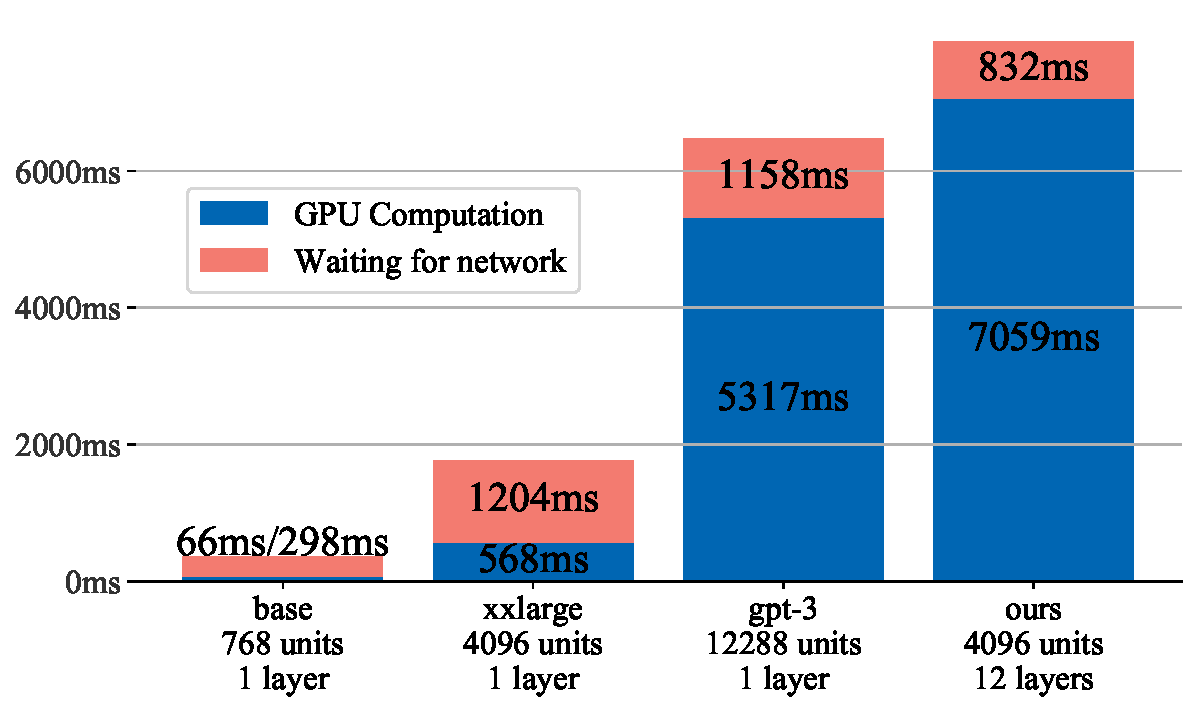
\includegraphics[width=1\linewidth]{resources/perf_absolute.pdf}
    \vspace{-12pt}
    \captionof{figure}{Pipeline computation and idle time per batch at 500 Mb/s bandwidth.}
    \label{fig:throughput_exps}
\end{figure}%
\begin{table}
    \centering
    \captionof{table}{Relative device utilization at 500 Mb/s bandwidth and varying network latency.}
    \label{tab:latency}
    \small
    \setlength{\tabcolsep}{8pt}
    \begin{tabular}[b]{@{}lcccc@{}}
    \toprule
    \multirow{2}{*}{\thead{Latency\\(RTT)}} & 
    \multicolumn{4}{c}{
    \thead{
    Relative GPU utilization\\ (100\% - idle time)
    }
    }
    
    \\
\cmidrule{2-5}                     & base & xxlarge & GPT-3 & Ours \\ \midrule
    None &   18.0\%     &  32.1\%         &  82.1\%  &  89.5\%      \\
    10ms &   11.8\%      &   28.9\%    &   79.3\%   &  87.2\%    \\
    50ms &    4.88\%      &   20.1\%    &   70.3\% &  79.5\%    \\
    100ms &    2.78\%      &    14.9\%    &  60.2\%     &   71.5\% \\
    200ms &   1.53\%     &  10.1\%    &  48.5\%   &     59.2\%    \\
    \bottomrule
    \end{tabular}
    \vspace{-6pt}
\end{table}

As depicted in Figure~\ref{fig:squarecube} (right) and Figure~\ref{fig:throughput_exps}, larger models achieve better GPU utilization rate in the same network conditions, since their communication load grows slower than computation. More importantly, even at 500 Mb/s, the resulting GPU idle time can be pushed into the 10--20\% range, either naturally for GPT-3-sized models or through activation compression for smaller models. In addition, large models maintain most of their training efficiency at the 100ms latency~(Table~\ref{tab:latency}), which is roughly equivalent to training on different continents~\citep{verizon_latency}.

\vspace{-4pt}
\subsection{Detailed Performance Comparison}\label{appendix:training_throughput}

Here we investigate how SWARM parallelism compares to existing systems for training large models: \textbf{GPipe}~\citep{huang2019gpipe} and \textbf{ZeRO-Offload}~\citep{zerooffload}.
The purpose of this section is to compare the training throughput in ``ideal'' conditions (with homogeneous reliable devices and balanced layers), as deviating from these conditions makes it \textit{infeasible} to train with baseline systems.
Still, even in such conditions the performance of different systems can vary across model architectures, and hence we want to identify the cases in which using SWARM is preferable to other approaches.
We benchmark individual SWARM components in preemptible setups in Section~\ref{sect:experiments_adaptive} and Appendix~\ref{appendix:scaling}.

We evaluate training performance for sequences of 4 Transformer layers of identical size distributed over 16 workers. Similarly to Section~\ref{sect:experiments_square_cube}, we use three layer configurations: ``xxlarge''~($d_{model} {=} 4096$, $d_{\text{FFN}} {=} 16384$, 32 heads), ``GPT-3''~($d_{model} {=} 12288$, $d_{\text{FFN}} {=} 49152$, 96 heads), and ``Ours''~($d_{model} {=} 4096$, $d_{\text{FFN}} {=} 16384$, 32 heads, 16 shared layers per block, last stage holds only the vocabulary projection layer). The microbatch size is 4 for ``xxlarge'' and 1 for ``GPT-3'' and ``Ours'', and the sequence length is 512.

To provide a more detailed view of the training performance, we measure two separate performance statistics: the training throughput and the All-Reduce time. 
The training throughput measures the rate at which the system can process training sequences, i.e., run forward and backward passes. 
More specifically, we measure the time required to process 6250 sequences of 512 tokens, which corresponds to the largest batch size used in~\citet{gpt3}.
In turn, the All-Reduce time is the time each system spends to aggregate accumulated gradients across devices. 
Intuitively, training with small batch sizes is more sensitive to the All-Reduce time (since the algorithm needs to run All-Reduce more frequently) and vice versa.


\textbf{Hardware setup:} Each worker uses a V100-PCIe GPU with 16 CPU threads (E5 v5-2660v4) and 128 GB RAM. The only exception is for ZeRO-Offload with ``GPT-3'' layers, where we had to double the RAM size because the system required 190 gigabytes at peak. Similarly to Section~\ref{sect:experiments_square_cube}, each worker can communicate at a 500 Mb/s bandwidth for both upload and download for a total of 1 Gb/s.
In terms of network latency, we consider two setups: with \textbf{no latency}, where workers communicate normally within the same rack, and with \textbf{latency}, where we introduce additional $100\pm50$ms latency directly in the kernel\footnote{More specifically, \texttt{tc qdisc add dev <...> root netem delay 100ms 50ms}}.

\textbf{GPipe configuration:} We use a popular PyTorch-based implementation of GPipe\footnote{The source code is available at \url{https://github.com/kakaobrain/torchgpipe}}. The model is partitioned into 4 stages repeated over 4 model-parallel groups. To fit into the GPU memory for the ``GPT-3'' configuration, we offload the optimizer into RAM using ZeRO-Offload. Before averaging, we use PyTorch's built-in All-Reduce to aggregate gradients.
We evaluate both the standard GPipe schedule and the 1F1B schedule~\citep{pipedream}.

\textbf{ZeRO-Offload configuration:} Each worker runs the entire model individually, then exchanges gradients with peers. For ``xxlarge'', we use the official implementation from~\cite{zerooffload}. However, for ``GPT-3'', we found that optimizer offloading still does not allow us to fit 4 layers into the GPU. For this reason, we also offload the model parameters using the \texttt{offload\_param} option.

\begin{table}
\centering
\small
\setlength{\tabcolsep}{4pt}
\captionof{table}{Training performance for different model sizes.}
\label{tab:throughput_gpt}
\begin{tabular}[b]{lcccc}
\toprule
\multirow{2}[2]{*}{System} &
  \multicolumn{2}{c}{Throughput, min/batch} &
  \multicolumn{2}{c}{All-Reduce time, min} \\ \cmidrule(lr){2-3}\cmidrule(lr){4-5} 
                 & No latency & Latency & No latency & Latency \\
 \midrule \multicolumn{5}{c}{``GPT-3'' (4 layers) }\\
 \midrule
SWARM            &  168.3 &\textbf{186.7}  &  7.4 & \textbf{7.6}   \\
GPipe            &  164.5 & 218.4 &  \multirow{2}{*}{\textbf{6.7}}    & \multirow{2}{*}{7.8}   \\
1F1B & \textbf{163.3} & 216.1 & & \\
Offload          &  272.7 & 272.7          &  25.5 & 27.3 \\
\midrule \multicolumn{5}{c}{``xxlarge'' (4 layers) }\\
\midrule
SWARM            &  44.2 & 48.2                  &  0.8  & \textbf{0.9}   \\
GPipe            &  40.1 & 108.8                  &  \multirow{2}{*}{\textbf{0.7}}  & \multirow{2}{*}{1.1}   \\
1F1B & 40.8 & 105.5 & & \\
Offload          &  \textbf{33.8} & \textbf{33.8}  &  2.8 & 4.2   \\
\midrule \multicolumn{5}{c}{Full ``Ours'' model (48 shared layers + embeddings) }\\
\midrule
SWARM            &  432.2 & 452.9                  &  0.8  &\bf 1.0   \\
GPipe            &  420.0 & 602.1                   &  \multirow{2}{*}{\bf 0.7}  & \multirow{2}{*}{1.1}   \\
1F1B             &  408.5 & 569.2 & & \\
Offload          &  \bf 372.0 &\bf 372.0  &  3.2 & 4.8   \\
\bottomrule
\end{tabular}
\vspace{-8pt}
\end{table}%

\begin{figure}[b]
\vspace{-16pt}
\centering
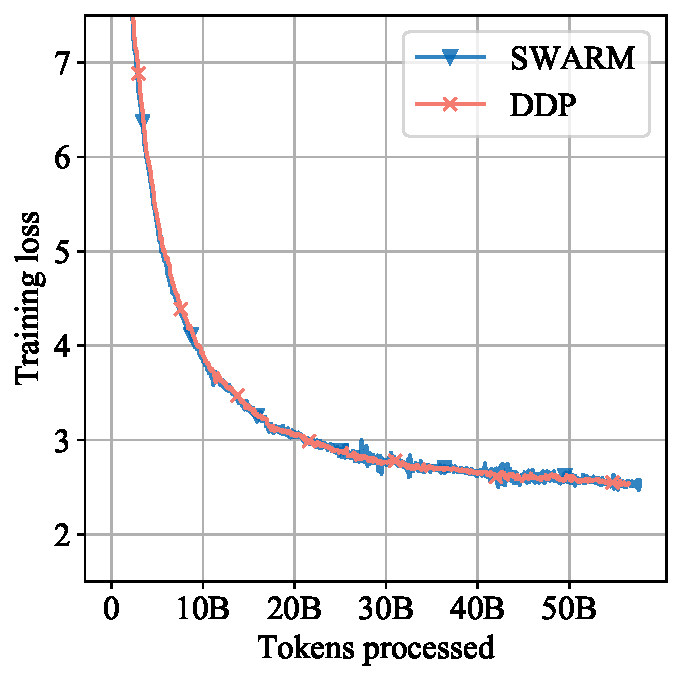
\includegraphics[ width=0.65\linewidth]{resources/learning_3stages.pdf}
\vspace{-6pt}
\captionof{figure}{Training convergence comparison.}
\label{fig:convergence}
\end{figure}

In turn, when training smaller models, ZeRO-Offload outperforms both SWARM and GPipe. This result aligns with our earlier observations in Figure~\ref{fig:squarecube}, where the same model spent most of the time waiting for the communication between pipeline stages.%

We also observe that ZeRO-Offload takes longer to aggregate gradients, likely because each peer must aggregate the entire model, whereas in SWARM and GPipe, peers aggregate a single pipeline stage. The variation between All-Reduce time in GPipe and SWARM is due to implementation differences. Overall, SWARM is competitive to HPC baselines even in an idealized homogeneous environment.

\subsection{Large-Scale Distributed Training}
\label{sect:experiments_large}

To verify the efficiency of SWARM parallelism in a practical scenario, we conduct a series of large-scale distributed experiments using preemptible (unreliable) cloud T4 and A100 GPUs over a public cloud network.

We train a Transformer language model with the architecture similar to prior work~\citep{gpt3,gptj,gptneo} and 1.01 billion parameters in total. Our model consists of 3 stages, each containing a single Transformer decoder block with $d_{model}=4096$ and 16 layers per pipeline stage. All workers within a stage serve the same group of layers, and all layers within each group use the same set of parameters, similarly to ALBERT~\citep{albert}. On top of this, the first stage also contains the embedding layer, and the last stage includes the language modeling head. Because of layer sharing, this model is equivalent to a 13B model from~\citet{gpt3} in terms of compute costs. 

We use 8-bit compression~\citep{adam8bit} for activations and gradients to reduce the communication intensity. Additional training setup details are covered in Appendix~\ref{appendix:detailed_large}.
SWARM nodes run rebalancing every $T=300$ seconds, and trainers measure peer performance using a moving average with $\alpha=0.1$. However, as we show in Section~\ref{sect:experiments_adaptive}, the throughput of SWARM is not very sensitive to the choice of these hyperparameters.



First, to verify that model parallelism with asynchronous updates does not have significant convergence issues, we train the model on the Pile~\citep{gao2020pile} dataset with 400 preemptible T4 instances, each hosting one accelerator. As a baseline, we use regular data-parallel training with offloading on 128 A100 GPUs.
We run both experiments for approximately 4 weeks and compare the learning curves.




Figure~\ref{fig:convergence} shows the results of this experiment: it can be seen that the training dynamics of two approaches are indeed similar, which demonstrates the viability of SWARM parallelism for heterogeneous and poorly-connected devices.

In the next experiment, we aim to measure the pipeline throughput in different hardware conditions and to compare it with an estimate of best-case pipeline performance.
We consider several setups: first, we use the same 400 preemptible T4 nodes; in another setup, we use 7 instances with 8 A100 GPU each; finally, we combine these fleets to create a heterogeneous setup. We examine the performance of the pipeline both with weight sharing and with standard, more common, Transformer blocks.

\begin{table}
\centering
\captionof{table}{Pipeline throughput, layer sharing.}
\label{tab:throughput}
\small
\begin{tabular}{@{}lcccc@{}}
\toprule
\multirow{2}{*}{\begin{tabular}[c]{@{}l@{}}Hardware\\ setup\end{tabular}} &
  \multicolumn{2}{c}{\begin{tabular}[c]{@{}c@{}}Throughput,\\ samples/s\end{tabular}} &
  \multicolumn{2}{c}{\begin{tabular}[c]{@{}c@{}}Optimal\\ bandwidth, Mb/s\end{tabular}} \\ \cmidrule(lr){2-3}\cmidrule(lr){4-5} 
                 & Actual & Best-case & Upload & Download \\ \midrule
T4           &  17.6      &   19.2        &   317.8     &     397.9     \\
A100          & 16.9       &   25.5        &   436.1     &     545.1     \\
T4 \& A100 &   27.3     &       ---    &   ---     &      ---    \\ \bottomrule
\end{tabular}
\end{table}
\begin{table}
\centering
\captionof{table}{Pipeline throughput, default Transformer.}
\label{tab:throughput_standard}
\small
\begin{tabular}{@{}lcc@{}}
\toprule
\multirow{2}{*}{\begin{tabular}[c]{@{}l@{}}Hardware\\ setup\end{tabular}} &
  \multicolumn{2}{c}{\begin{tabular}[c]{@{}c@{}}Throughput,\\ samples/s\end{tabular}} \\ \cmidrule(lr){2-3}
                 & Actual & Best-case \\ \midrule
T4           &  8.8      &   19.3        \\
A100          & 8.0       &   25.1        \\
T4 \& A100 &   13.4     &       ---    \\ \bottomrule
\end{tabular}
\end{table}






We measure the number of randomly generated samples processed by the pipeline both in our infrastructure and the ideal case that ignores all network-related operations (i.e., has infinite bandwidth and zero latency). The ideal case is emulated by executing a single pipeline stage 3 times locally on a single server and multiplying the single-node estimates by the number of nodes.

As demonstrated in the left two columns of Table~\ref{tab:throughput} and Table~\ref{tab:throughput_standard}, asynchronous training of compute-intensive models with 8-bit compressed activations regardless of the architecture specifics allows us to achieve high performance without a dedicated networking solution. Furthermore, the load balancing algorithm of SWARM allows us to dynamically and efficiently utilize different hardware without being bottlenecked by slower devices. 


Next, we use the same load testing scenario to estimate the bandwidth required to fully utilize each device type in the above infrastructure. For this, we measure the average incoming and outgoing bandwidth on the nodes that serve the intermediate stage of the pipeline. We summarize our findings in the right two columns of Table~\ref{tab:throughput}: it turns out that with layer sharing and 8-bit compression, medium-performance GPUs (such as T4) can be saturated even with moderate network speeds. Based on our main experiment, the optimal total bandwidth is roughly 100Mb/s higher than the values reported in Table 3 due to gradient averaging, loading state from peers, maintaining the DHT and streaming the training data.
Although training over the Internet with more efficient hardware might indeed underutilize the accelerator, this issue can be offset by advanced compression strategies such as compression-aware architectures or layer sharing, as shown in Table~\ref{tab:throughput}.

\begin{figure}[t]
    \centering
    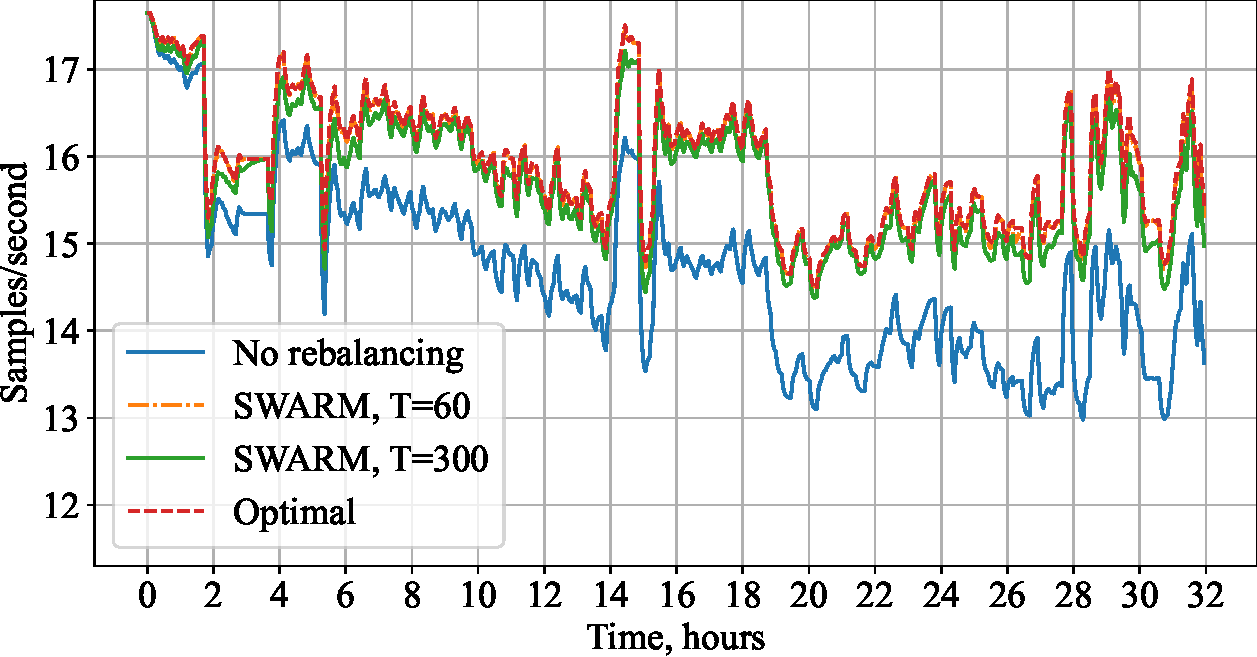
\includegraphics[width=\linewidth]{resources/rebalancing_activity.pdf}
    \captionof{figure}{Throughput of rebalancing methods over time.}
    \label{fig:rebalancing}
\end{figure}

\subsection{Adaptive Rebalancing Evaluation}


\begin{figure*}[h!]
\begin{subfigure}{0.5\textwidth}
    \centering
    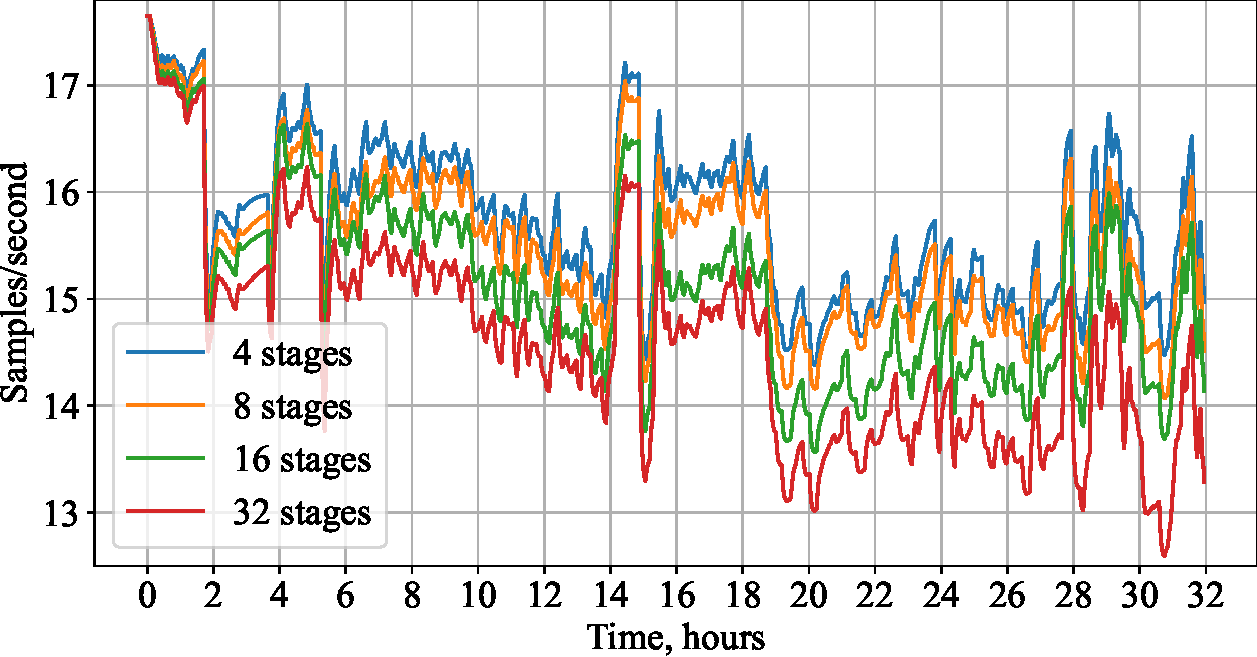
\includegraphics[width=0.97\linewidth]{resources/rebalancing_stages.pdf}
    \caption{Adaptive rebalancing of SWARM parallelism.}
    \label{fig:rebalancing_stages}
\end{subfigure}%
\begin{subfigure}{0.5\textwidth}
    \centering
    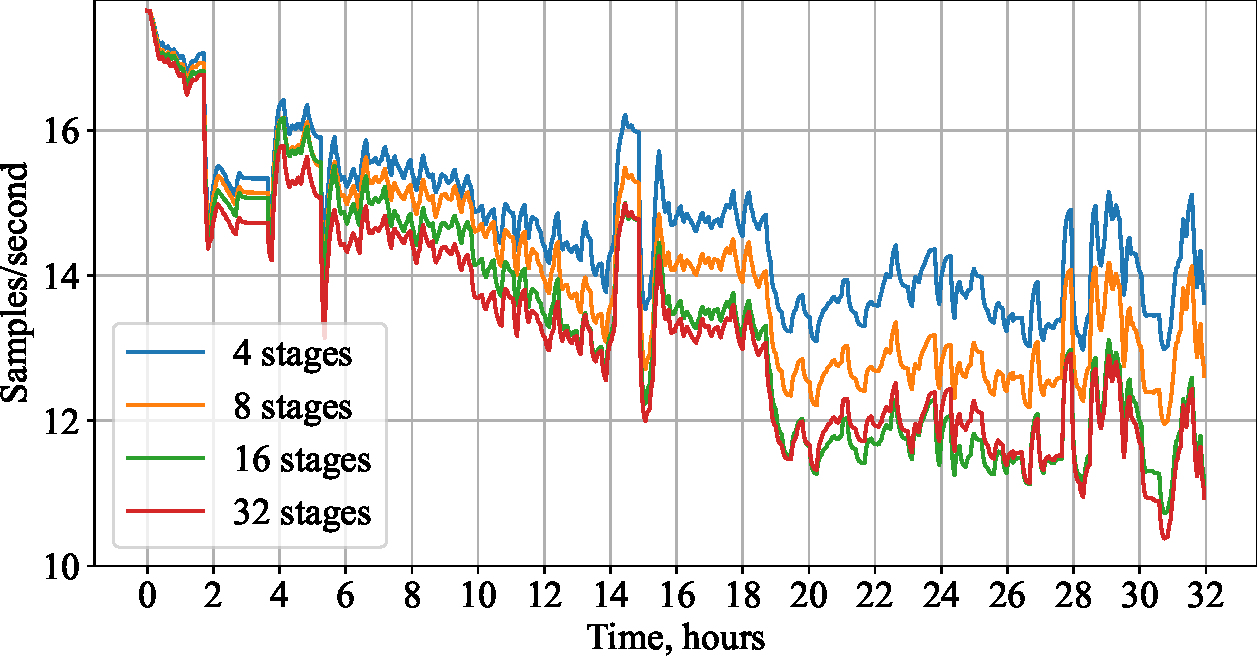
\includegraphics[width=0.97\linewidth]{resources/rebalancing_stages_baseline.pdf}
    \caption{No rebalancing.}
    \label{fig:rebalancing_stages_baseline}
\end{subfigure}
\caption{Scaling of pipeline-parallel strategies with respect to the number of stages.}
\label{fig:rebalancing_stages_all}
\end{figure*}

\label{sect:experiments_adaptive}
In this experiment, we evaluate the efficiency of adaptive peer rebalancing between stages proposed in Section~\ref{sect:method_swarm}. 
We use statistics of the number of active T4 nodes from the 32-hour segment of the experiment described in Section~\ref{sect:experiments_large}. 
We use this data to simulate training dynamics by viewing it as sequence of events, each consisting of a timestamp and a change in the number of peers (which can be positive or negative). 
When a worker is removed from the pipeline, we randomly choose the stage it was removed from: that is, removing $N$ peers corresponds to $N$ samples from the uniform distribution over four pipeline stages. 
We run 10 simulations with different random seeds and average the resulting trajectories.
We compare our strategy with two different values of $T$ to the baseline that has no rebalancing.

The results of this evaluation are available in \autoref{fig:rebalancing}; for reference, we also provide the performance of a theoretically optimal rebalancing strategy that maintains the highest possible throughput at every moment. It can be seen that even with the rebalancing period $T=300$, our approach significantly improves the overall throughput of the pipeline. When the number of peers is relatively stable, the rebalanced pipeline also approaches the optimal one in terms of throughput, which shows the efficiency of rebalancing even when moving only one node at a time.

In addition, we observed that for some brief periods, the performance of the unbalanced pipeline exceeded the throughput of the balanced one due to random choice of disconnecting peers (dropping more from the ``overrepresented'' stages affects the imbalanced pipeline less). However, this held true only for $\approx 4.5\%$ of the experiment and was quickly mitigated by adaptive rebalancing.

As expected, decreasing $T$ from 300 to 60 seconds improves both the overall throughput and the speed of convergence to optimal pipeline performance. However, the effect is not as drastic compared to the increase in DHT data transfer volume. This is also demonstrated by \autoref{tab:rebalancing_speedup}, which shows the relative throughput of the three configurations compared to the optimal one. Furthermore, the table displays that while initially there is little difference between rebalancing choices, it becomes more pronounced later on as the imbalanced version ``drifts further'' from the optimal state.

\begin{table}[b]
\centering
\captionof{table}{Relative throughput comparison of pipeline rebalancing methods.}
\small
\label{tab:rebalancing_speedup}
\begin{tabular}[b]{@{}lccc@{}}
\toprule
\multirow{2}[2]{*}{\thead{Rebalancing}} & \multicolumn{3}{c}{\% of optimal} \\ \cmidrule(l){2-4} 
                        & Overall   & First 1 hour   & Last 1 hour  \\ \midrule
None                & 82.7      & 99.0       & 45.4     \\
$T=300$    & 95.8      & 99.4       & 88.9     \\
$T=60$     & 97.6      & 99.8       & 91.7     \\ \bottomrule
\end{tabular}
\end{table}

Finally, we analyze the scaling properties of rebalancing with respect to the number of stages. To do this, we conduct experiments in the same setup as above ($T=300$) while changing the number of pipeline stages from 4 to $\{4,\ 8,\ 16,\ 32\}$. To ensure the consistency of throughput across all experiments, we increase the starting number of peers accordingly while keeping the preemption rate constant. As a baseline, we also evaluate the throughput of the pipeline that has no rebalancing.

Figure~\ref{fig:rebalancing_stages_all} shows the outcome of this experiment. As displayed in the plots, both strategies drop in performance with the increase in the stage count: while all stages should drop in performance equally in expectation, in practice, the variances are too large while the number of peers is relatively too small for the asymptotic properties to take place. This effect results in more outliers (large drops in the number of peers) in the preemption distribution for more stages. Still, rebalancing allows to partially mitigate the issue: while we observe a more consistent downward trend for the baseline strategy, the rebalanced pipeline regains its performance over time and achieves a higher overall throughput.


\section{Conclusions}
\label{conclusions}

In this paper a modification of the unsupervised Isolation Forest named \approach has been suggested to improve the performance of the standard algorithm.
Due to the lack of fully labelled datasets, Anomaly Detection is often performed by means of unsupervised models. However, as anomalies heavily depend on the context and are very domain specific, unsupervised models may be unable to detect them because of different definition of anomaly.
To solve this problem we suggest a model that starting from an unsupervised model, iteratively tunes the model towards the user-definition of anomaly. This allows to enhance the detection performances, avoiding the need to fully label the training dataset and keeping as low as possible the number of required labels. Indeed this approach  takes advantage of the Active Learning framework where the model is able to query the user and select the most interesting samples to label.
\approach relies on two important and inter-connected steps: the query policy that selects the point to be labelled, and the model update policy that allows the model to actually learn from the new query. 
From experiments performed on real datasets  it turned out it is better to ask to label the most anomalous point, leading to a cheap and natural query strategy in practice. Concerning the update policy, the model does not need to fully retrain the forest, but needs just a simple update of the leaf depth, with a cost $O(n_T)$. Regarding the query strategy, the required cost is $O(n_X n_T)$. The cheap time complexity together with the fact that \approach does not need labels of both anomalies and normal points provides a great advantage compared to other state-of-art algorithms.
Comparing \approach with other methods, it turns out it is also generally much faster in the learning of the correct anomaly definition, when the labelling effort needs to be kept low.

Future works will investigate the different query and updating strategies: the information of the number of data points in each leaf might be included in the algorithm, to estimate the uncertainty on the leaf depth correction. Moreover, hybrid query strategies that use a combination of the previously described, might lead to even better results.


\section*{Acknowledgement}
This work has been supported by MIUR (Italian Minister for Education) under the initiative “Departments of Excellence” (Law 232/2016) and by "Black-box Anomaly Detection: Advanced Approaches and Applications - BADA$^3$" funded by the Department of Information Engineering of University of Padova.

\bibliography{bibliography.bib}


\end{document}
